%!TEX TS-program = xelatex
\documentclass[notes,12pt, aspectratio=169]{beamer}

\usepackage{amsmath,amsfonts,amssymb,amsthm,mathtools}  % пакеты для математики
\usepackage{minted}

\usepackage[english, russian]{babel} % выбор языка для документа
\usepackage[utf8]{inputenc} % задание utf8 кодировки исходного tex файла
\usepackage[X2,T2A]{fontenc}        % кодировка

\usepackage{fontspec}         % пакет для подгрузки шрифтов
\setmainfont{Helvetica}  % задаёт основной шрифт документа

% why do we need \newfontfamily:
% http://tex.stackexchange.com/questions/91507/
\newfontfamily{\cyrillicfonttt}{Helvetica}
\newfontfamily{\cyrillicfont}{Helvetica}
\newfontfamily{\cyrillicfontsf}{Helvetica}

\usepackage{unicode-math}     % пакет для установки математического шрифта
% \setmathfont{Neo Euler} % шрифт для математики

\usepackage{polyglossia}      % Пакет, который позволяет подгружать русские буквы
\setdefaultlanguage{russian}  % Основной язык документа
\setotherlanguage{english}    % Второстепенный язык документа

% Шрифт для кода
\setmonofont[Scale=0.85]{Monaco}
\usepackage{verbments}

\usepackage{pgfpages}
% These slides also contain speaker notes. You can print just the slides,
% just the notes, or both, depending on the setting below. Comment out the want
% you want.
%\setbeameroption{hide notes} % Only slide
%\setbeameroption{show only notes} % Only notes
%\setbeameroption{show notes on second screen=right} % Both

\usepackage{array}

\usepackage{tikz}
\usepackage{verbatim}
\setbeamertemplate{note page}{\pagecolor{yellow!5}\insertnote}
\usetikzlibrary{positioning}
\usetikzlibrary{snakes}
\usetikzlibrary{calc}
\usetikzlibrary{arrows}
\usetikzlibrary{decorations.markings}
\usetikzlibrary{shapes.misc}
\usetikzlibrary{matrix,shapes,arrows,fit,tikzmark}

\usepackage{hyperref}
\usepackage{lipsum}
\usepackage{multimedia}
\usepackage{multirow}
\usepackage{dcolumn}
\usepackage{bbm}
\newcolumntype{d}[0]{D{.}{.}{5}}

\usepackage{changepage}
\usepackage{appendixnumberbeamer}
\newcommand{\beginbackup}{
   \newcounter{framenumbervorappendix}
   \setcounter{framenumbervorappendix}{\value{framenumber}}
   \setbeamertemplate{footline}
   {
     \leavevmode%
     \hline
     box{%
       \begin{beamercolorbox}[wd=\paperwidth,ht=2.25ex,dp=1ex,right]{footlinecolor}%
%         \insertframenumber  \hspace*{2ex} 
       \end{beamercolorbox}}%
     \vskip0pt%
   }
 }
\newcommand{\backupend}{
   \addtocounter{framenumbervorappendix}{-\value{framenumber}}
   \addtocounter{framenumber}{\value{framenumbervorappendix}} 
}

% для имитации питоновского синтаксиса 
\newcommand{\pgr}[1]{{\color{green} \textbf{#1}}}


%%%%%%%%%% Работа с картинками %%%%%%%%%
\usepackage{graphicx}                  % Для вставки рисунков
\usepackage{graphics}
\graphicspath{{images/}}    % можно указать папки с картинками
\usepackage{wrapfig}                   % Обтекание рисунков и таблиц текстом

\usepackage[space]{grffile}
\usepackage{booktabs}

% These are my colors -- there are many like them, but these ones are mine.
\definecolor{blue}{RGB}{0,114,178}
\definecolor{red}{RGB}{213,94,0}
\definecolor{yellow}{RGB}{240,228,66}
\definecolor{green}{RGB}{0,128, 0}

\hypersetup{
  colorlinks=true,
  linkbordercolor = {white},
  linkcolor = {blue},
  urlcolor= {blue}
}


%% I use a beige off white for my background
\definecolor{MyBackground}{RGB}{255,253,218}

%% Uncomment this if you want to change the background color to something else
%\setbeamercolor{background canvas}{bg=MyBackground}

%% Change the bg color to adjust your transition slide background color!
\newenvironment{transitionframe}{
  \setbeamercolor{background canvas}{bg=yellow}
  \begin{frame}}{
    \end{frame}
}

\setbeamercolor{frametitle}{fg=blue}
\setbeamercolor{title}{fg=black}
\setbeamertemplate{footline}[frame number]
\setbeamertemplate{navigation symbols}{} 
\setbeamertemplate{itemize items}{-}
\setbeamercolor{itemize item}{fg=blue}
\setbeamercolor{itemize subitem}{fg=blue}
\setbeamercolor{enumerate item}{fg=blue}
\setbeamercolor{enumerate subitem}{fg=blue}
\setbeamercolor{button}{bg=MyBackground,fg=blue,}


% If you like road maps, rather than having clutter at the top, have a roadmap show up at the end of each section 
% (and after your introduction)
% Uncomment this is if you want the roadmap!
% \AtBeginSection[]
% {
%    \begin{frame}
%        \frametitle{Roadmap of Talk}
%        \tableofcontents[currentsection]
%    \end{frame}
% }
\setbeamercolor{section in toc}{fg=blue}
\setbeamercolor{subsection in toc}{fg=red}
\setbeamersize{text margin left=1em,text margin right=1em} 

% списки, которые растягиваются на всю величину слайда 
\newenvironment{wideitemize}{\itemize\addtolength{\itemsep}{10pt}}{\enditemize}


\usepackage{xcolor}

% Syntax: \colorboxed[<color model>]{<color specification>}{<math formula>}
\newcommand*{\colorboxed}{}
\def\colorboxed#1#{%
	\colorboxedAux{#1}%
}

\newcommand*{\colorboxedAux}[3]{%
	% #1: optional argument for color model
	% #2: color specification
	% #3: formula
	\begingroup
	\colorlet{cb@saved}{.}%
	\color#1{#2}%
	\boxed{%
		\color{cb@saved}%
		#3%
	}%
	\endgroup
}

\usepackage{pgfplots}
\usepackage{tikz}

\DeclareMathOperator{\logloss}{logloss}

\title[]{\textcolor{blue}{Глубокое обучение и вообще}}
\author{Ульянкин Филипп}
\date{\today}

\usepackage{ulem}

\begin{document}

%%% TIKZ STUFF
\tikzset{   
        every picture/.style={remember picture,baseline},
        every node/.style={anchor=base,align=center,outer sep=1.5pt},
        every path/.style={thick},
        }
\newcommand\marktopleft[1]{%
    \tikz[overlay,remember picture] 
        \node (marker-#1-a) at (-.3em,.3em) {};%
}
\newcommand\markbottomright[2]{%
    \tikz[overlay,remember picture] 
        \node (marker-#1-b) at (0em,0em) {};%
}
\tikzstyle{every picture}+=[remember picture] 
\tikzstyle{mybox} =[draw=black, very thick, rectangle, inner sep=10pt, inner ysep=20pt]
\tikzstyle{fancytitle} =[draw=black,fill=red, text=white]
%%%% END TIKZ STUFF

% Title Slide

\begin{frame}
\maketitle
\centering \textbf{\color{blue} Посиделка 3:}  50 оттенков градиентного спуска
\end{frame}

\begin{frame}{Agenda}
\begin{wideitemize}
	\item 50 оттенков градиентного спуска
	% \item Матричное дифференцирование 
	\item Начнём потихоньку разбираться с алгоритмом обратного распространения ошибки
\end{wideitemize} 
\end{frame}

\begin{transitionframe}
	\begin{center}
		\Huge 50 оттенков градиентного спуска
	\end{center}
\centering 
\includegraphics[scale = 0.1]{shadows50.jpg}
\end{transitionframe}

\begin{frame}{Как обучать нейросеть?}
\begin{wideitemize}
	\item  Нейросеть - сложная функция, зависящая от весов $W$ 
	\item «Тренировка» — поиск оптимальных $W$ 
	\item «Оптимальных» — минимизирующих какой-то функционал 
	\item Какими бывают функционалы: MSE, MAE, logloss и многие другие 
	\item Как оптимизировать: \alert{градиентный спуск!} 
\end{wideitemize} 
\end{frame}


\begin{frame}[fragile]{Градиентный спуск (GD)}
Проблема оптимизации: 

\[   
L(w) = \frac{1}{n} \cdot \sum_{i=1}^n L(w, x_i, y_i) \to \min_{w}
\]

\pause
Градиент указывает направление максимального роста

\[   
\nabla L(w) = \left( \frac{\partial L(w)}{\partial w_0},  \frac{\partial L(w)}{\partial w_2}, \ldots, \frac{\partial L(w)}{\partial w_k} \right)
\]

\pause 
Идём в противоположную сторону: 

\[
w^1 =  \underset{{\color{red} \text{скорость обучения}}}{ w^0 -   {\color{red} \eta }\cdot \nabla L(w^0)} 
\]
\end{frame}


\begin{frame}[fragile]{Градиентный спуск (GD)}
Проблема оптимизации: 

\[   
L(w) = \sum_{i=1}^n L(w, x_i, y_i) \to \min_{w}
\]

Инициализация $w_0$ 
\mint{python}{while True:}
\hspace{15pt} $g_t = \frac{1}{n}\sum_{i=1}^n  \nabla L(w, x_i, y_i)$ \\
\pgr{\hspace{15pt}} $w_t = w _{t-1} - \eta_t \cdot g_t $ \\
\pgr{\hspace{15pt} if} $||w_t - w_{t-1}|| < \varepsilon:$ \\
\pgr{\hspace{30pt} break}
\end{frame}


\begin{frame}{Градиентный спуск}
\begin{center}
	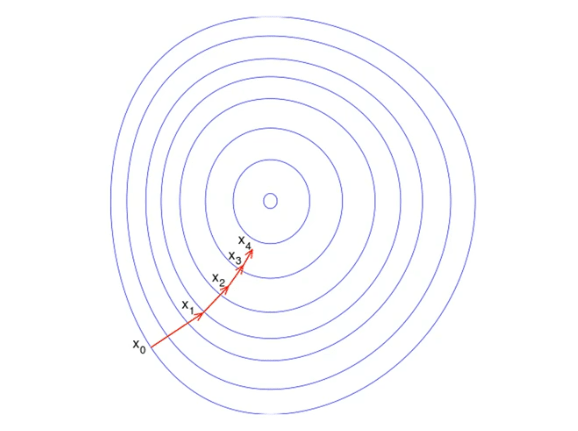
\includegraphics[width=.6\linewidth]{2dgrad.png}
\end{center}
\end{frame}


\begin{frame}[fragile]{Пример:}
Проблема оптимизации: 
\[   
L(w) = \frac{1}{n} \cdot \sum_{i=1}^n  (y_i - x_i^T w)^2 \to \min_{w}
\]

Градиент: 

\[   
\nabla L(w) =   { \only<2>{ \color{red}} -2 \cdot   \frac{1}{n} \cdot \sum_{i=1}^n (y_i - x_i^T w)\cdot x_i }
\]

Идём в противоположную сторону: 

\[
w^1 =   w^0  +  0.001 \cdot  { \only<2>{ \color{red}}  2 \cdot \frac{1}{n} \cdot \sum_{i=1}^n (y_i - x_i^T w)\cdot x_i } 
\]

\only<2>{ { \color{red} Дорого постоянно считать такие суммы!}}
\end{frame}


\begin{frame}[fragile]{Стохастический градиентный спуск (SGD)}
Проблема оптимизации: 

\[   
L(w) = \sum_{i=1}^n L(w, x_i, y_i) \to \min_{w}
\]

Инициализация $w_0$ 
\mint{python}{while True:}
\hspace{15pt} рандомно выбрали $i$ \\
\pgr{\hspace{15pt}} $g_t = \nabla L(w_{t-1}, x_i, y_i)$ \\
\pgr{\hspace{15pt}} $w_t = w _{t-1} - \eta_t \cdot g_t  $ \\
\pgr{\hspace{15pt} if} $||w_t - w_{t-1}|| < \varepsilon:$ \\
\pgr{\hspace{30pt} break}
\end{frame}



\begin{frame}[fragile]{Пример:}
Проблема оптимизации: 
\[   
L(w) = \frac{1}{n} \cdot \sum_{i=1}^n  (y_i - x_i^T w)^2 \to \min_{w}
\]

Градиент: 

\[   
\nabla L(w) =  { \color{red} - 2 \cdot (y_i - x_i^T w)\cdot x_i }
\]

Идём в противоположную сторону: 

\[
w^1 =   w^0  +  0.001 \cdot   {\color{red}  2 \cdot (y_i - x_i^T w_0)\cdot x_i }
\]
\end{frame}


\begin{frame}{Стохастический градиентный спуск (SGD)}
\begin{columns}[T] %
	\begin{column}{.5\textwidth}
		\resizebox{0.95\linewidth}{!}{
			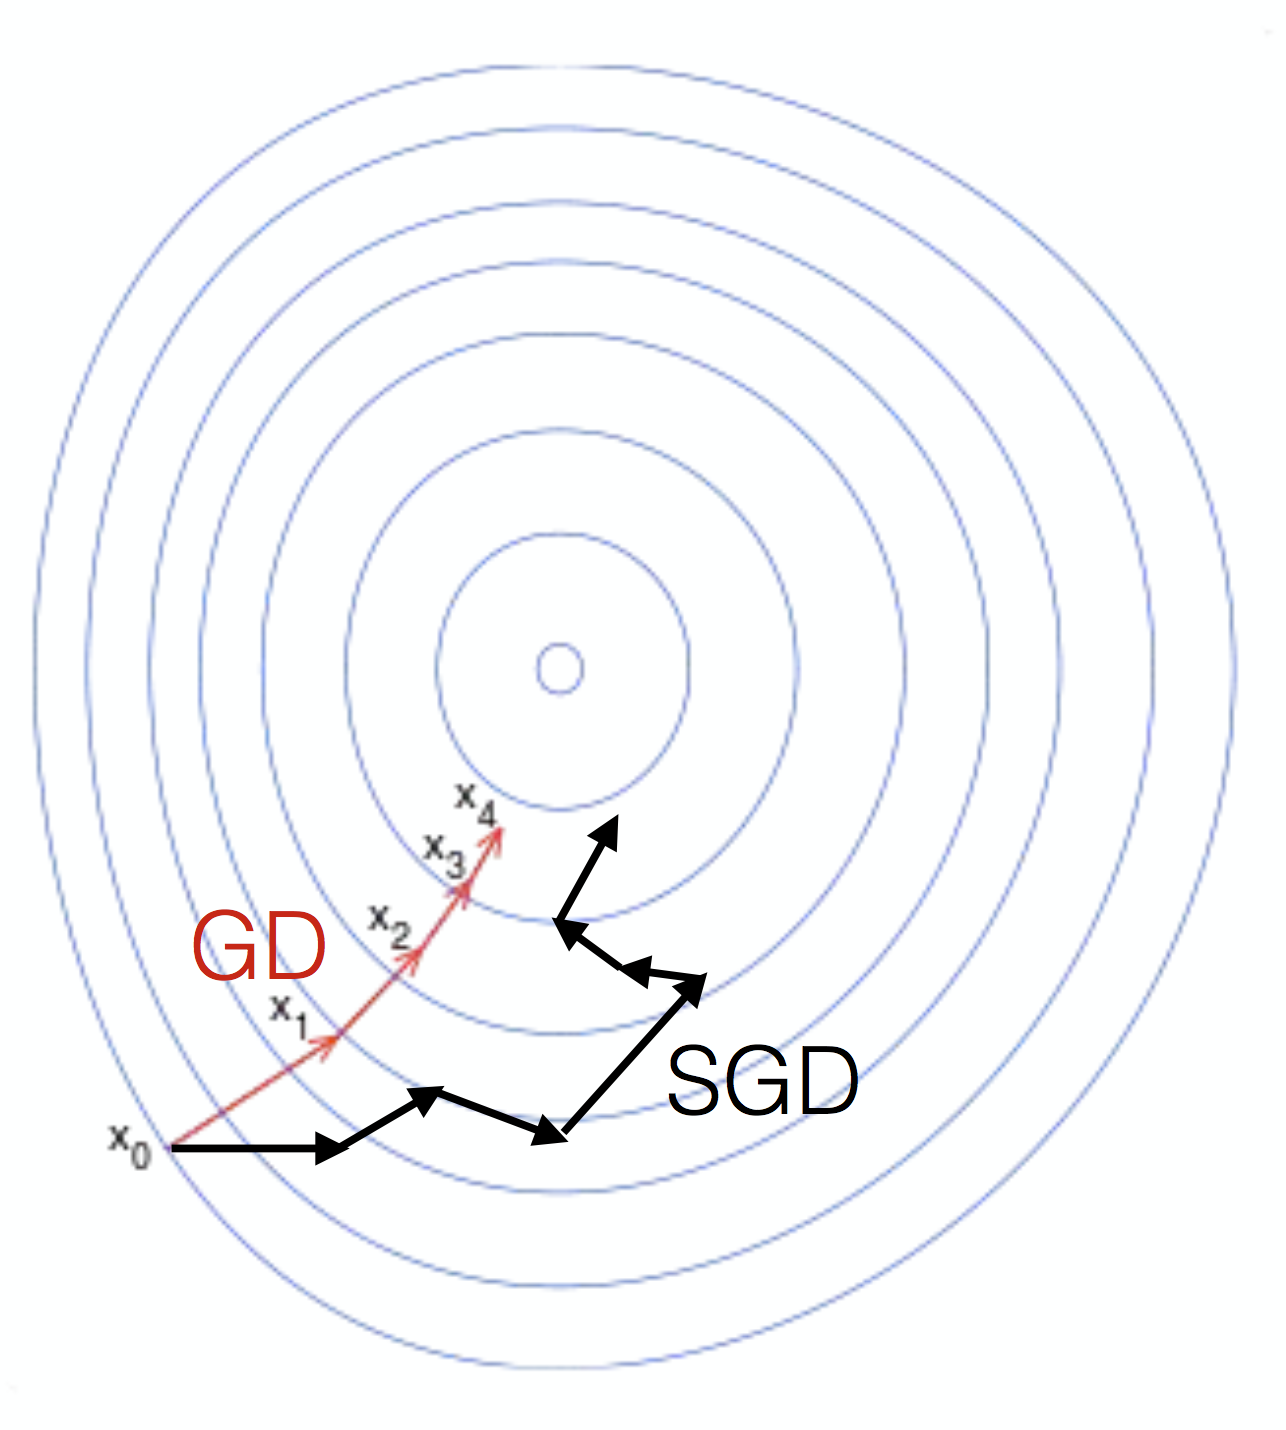
\includegraphics{st2grad.png}
		}
	\end{column}%
	\hfill%
	\begin{column}{.5\textwidth}
		\begin{wideitemize}
			\item И для GD и для SGD нет гарантий глобального минимума, сходимости
			\item SGD быстрее,на каждой итерации используется только одно наблюдение
			\item Для SGD спуск очень зашумлён 
			\item  GD: $O(n)$, SGD: $O(1)$
			\item Шум в оценке градиента помогает выпрыгивать из локальных оптимумов
		\end{wideitemize}
	\end{column}%
\end{columns}
\end{frame}


\begin{frame}[fragile]{Mini-bath SGD}
Проблема оптимизации: 

\[   
L(w) = \sum_{i=1}^n L(w, x_i, y_i) \to \min_{w}
\]

Инициализация $w_0$ 
\mint{python}{while True:}
\pgr{\hspace{15pt}} рандомно выбрали $m < n$ индексов \\
\pgr{\hspace{15pt}} $g_t =\frac{1}{m}\sum_{i=1}^m  \nabla L(w, x_i, y_i)$ \\
\pgr{\hspace{15pt}} $w_t = w _{t-1} - \eta_t \cdot g_t   $ \\
\pgr{\hspace{15pt} if} $||w_t - w_{t-1}|| < \varepsilon:$ \\
\pgr{\hspace{30pt} break}
\end{frame}


\begin{frame}[fragile]{Вызовы}
\begin{wideitemize}
	\item Скорость обучения $\eta$ надо подбирать аккуратно, если она будет большой, мы можем скакать вокруг минимума, если маленькой - вечно ползти к нему.
	
	\begin{center}
		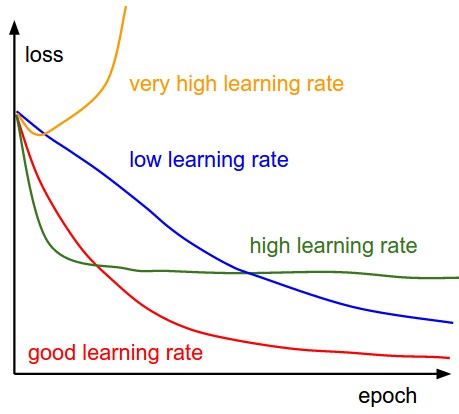
\includegraphics[width=0.25\paperwidth]{learningrates.jpg}
	\end{center}
	
	\item К обновлению всех параметров применяется одна и та же скорость обучения. Возможно, что какие-то параметры приходят в оптимальную точку быстрее, и их не надо обновлять.
\end{wideitemize}
\end{frame}



\begin{frame}{Momentum SGD}

Мы считали на каждом шаге градиент по формуле  \[g_t =\frac{1}{m}\sum_{i=1}^m  \nabla L(w_{t-1}, x_i, y_i).\] После шага мы забывали его. {\color{red} Давайте запоминать направление:} 

\begin{equation*}
	\begin{aligned}
	h_t &= \alpha \cdot h_{t-1} + \eta \cdot g_t \\
	w_t &= w_{t-1} - h_t
	\end{aligned}	
\end{equation*}

\begin{itemize}
	\item Движение поддерживается в том же направлении, что и на предыдущем шаге
	\item Нет резких изменений направления движения.
	\item Обычно $\alpha = 0.9$.
\end{itemize}

\vfill
\footnotesize
Крутой интерактив для моментума: {\color{blue} \url{https://distill.pub/2017/momentum/}}
\end{frame}


\begin{frame}{Momentum SGD}
\begin{wideitemize}
	\item Бежим с горки и всё больше ускоряемся в том направлении, в котором были направлены сразу несколько предыдущих градиентов, но при этом движемся медленно там, где градиент постоянно меняется
	\item Хотелось бы не просто бежать с горы, но и хотя бы на полшага смотреть себе под ноги, чтобы внезапно не споткнуться $\Rightarrow$  \alert{давайте смотреть на градиент в будущей точке}
	\item Согласно методу моментов $\alpha \cdot h_{t-1}$ точно будет использоваться при шаге, давайте искать $\nabla L(w_{t-1} - \alpha \cdot h_{t-1})$.
\end{wideitemize}
\end{frame}


\begin{frame}{Nesterov Momentum SGD}

\begin{itemize}
\item Мы теперь сначала прыгаем в том же направлении, в каком шли до этого, потом корректируем его (голубая траектория).
\end{itemize}

\begin{center}
	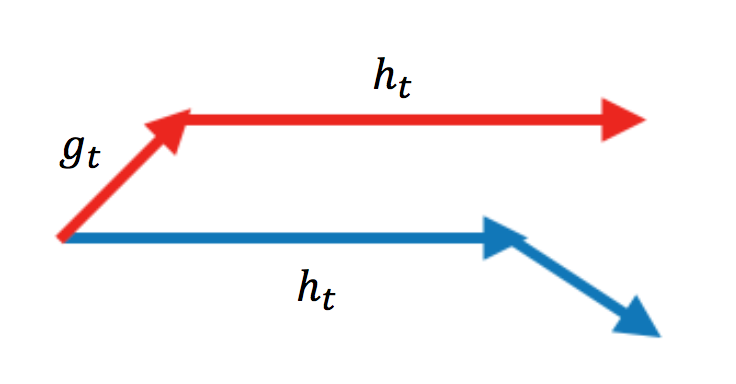
\includegraphics[width=.4\linewidth]{nesterov.png}
\end{center}

\begin{equation*}
\begin{aligned}
h_t &= \alpha \cdot h_{t-1} + \eta \cdot \nabla L(w_{t-1} - \alpha \cdot h_{t-1}) \\
w_t &= w_{t-1} - h_t
\end{aligned}	
\end{equation*}

\end{frame}


\begin{frame}{Разная скорость обучения}
\begin{wideitemize}
	\item Может сложиться, что некоторые веса уже близки к своим локальным минимумам, по этим координатам надо двигаться медленнее, а по другим быстрее $\Rightarrow$ {\color{red} адаптивные методы градиентного спуска }

	\item Шаг изменения должен быть меньше у тех параметров, которые в большей степени варьируются в данных, и больше у тех, которые менее изменчивы 
\end{wideitemize}
\end{frame}


\begin{frame}{AdaGrad}
\begin{equation*}
\begin{aligned}
G_t^j &= G_{t-1}^j + g_{tj}^2 \\
w_t^j &= w_{t-1}^j - \frac{\eta}{\sqrt{G_t^j + \varepsilon}} \cdot g_t^j
\end{aligned}	
\end{equation*}

\begin{wideitemize}
	\item  $g_t^j$ — градиент по $j-$ому параметру
	\item своя скорость обучения для каждого параметра
	\item обычно $\eta = 0.01$, т.к. параметр не очень важен
	\item $G_t^j$ всегда увеличивается, из-за этого обучение может рано останавливаться $\Rightarrow$  RMSprop
\end{wideitemize}
\end{frame}


\begin{frame}{RMSprop}
\begin{equation*}
\begin{aligned}
G_t^j &= \alpha \cdot G_{t-1}^j + (1 - \alpha) \cdot g_{tj}^2 \\
w_t^j &= w_{t-1}^j - \frac{\eta_t}{\sqrt{G_t^j + \varepsilon}} \cdot g_t^j
\end{aligned}	
\end{equation*}

\begin{wideitemize}
	\item Обычно $ \alpha = 0.9$
	\item Скорость обучения адаптируется к последнему сделанному шагу, бесконтрольного роста $G_t^j$ больше не происходит 
	\item RMSprop нигде не был опубликован, Хинтон просто привёл его в своей лекции, сказав, что это норм тема
\end{wideitemize}
\end{frame}


\begin{frame}{Adam (Adaptive Moment Estimation)}
\begin{equation*}
\begin{aligned}
h_t^j &= \beta_1 \cdot h_{t-1}^j + (1 - \beta_1) \cdot g_{tj} \\
G_t^j &= \beta_2 \cdot G_{t-1}^j + (1 - \beta_2) \cdot g_{tj}^2 \\
w_t^j &= w_{t-1}^j - \frac{\eta_t}{\sqrt{G_t^j + \varepsilon}} \cdot h_t^j
\end{aligned}	
\end{equation*}

\begin{wideitemize} 
\item Комбинируем Momentum и индивидуальные скорости обучения

\item Фактически $h_t$ и $G_t$ это оценки первого и второго моментов для стохастического градиента
\end{wideitemize}
\end{frame}


\begin{frame}{Сравнение на MNIST}
\begin{center}
	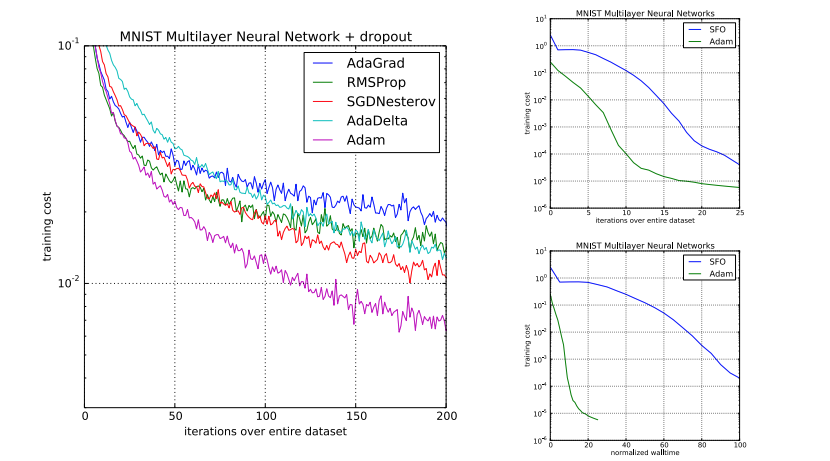
\includegraphics[scale=0.4]{adam_mnist.png}
\end{center}

\vfill %
\footnotesize
 {\color{blue} \url{https://arxiv.org/pdf/1412.6980.pdf}}
\end{frame}


\begin{frame}{Резюме по методам градиентного спуска}
\begin{wideitemize}
	\item Momentum SGD сохраняет направление шага и позволяет добиваться более быстрой сходимости
	
	\item  Адаптивные методы позволяют находить индивидуальную скорость обучения для каждого параметра
	
	\item Adam комбинирует в себе оба подхода
	
	\item Давайте посмотрим \href{http://ruder.io/content/images/2016/09/contours_evaluation_optimizers.gif}{визуализацию 1} и \href{http://ruder.io/content/images/2016/09/saddle_point_evaluation_optimizers.gif}{визуализацию 2}
	
	\item \alert{Но это же не все вызовы!} 
\end{wideitemize}
\end{frame}


\begin{frame}{Боб чилит в локальном минимуме}
\begin{center}
	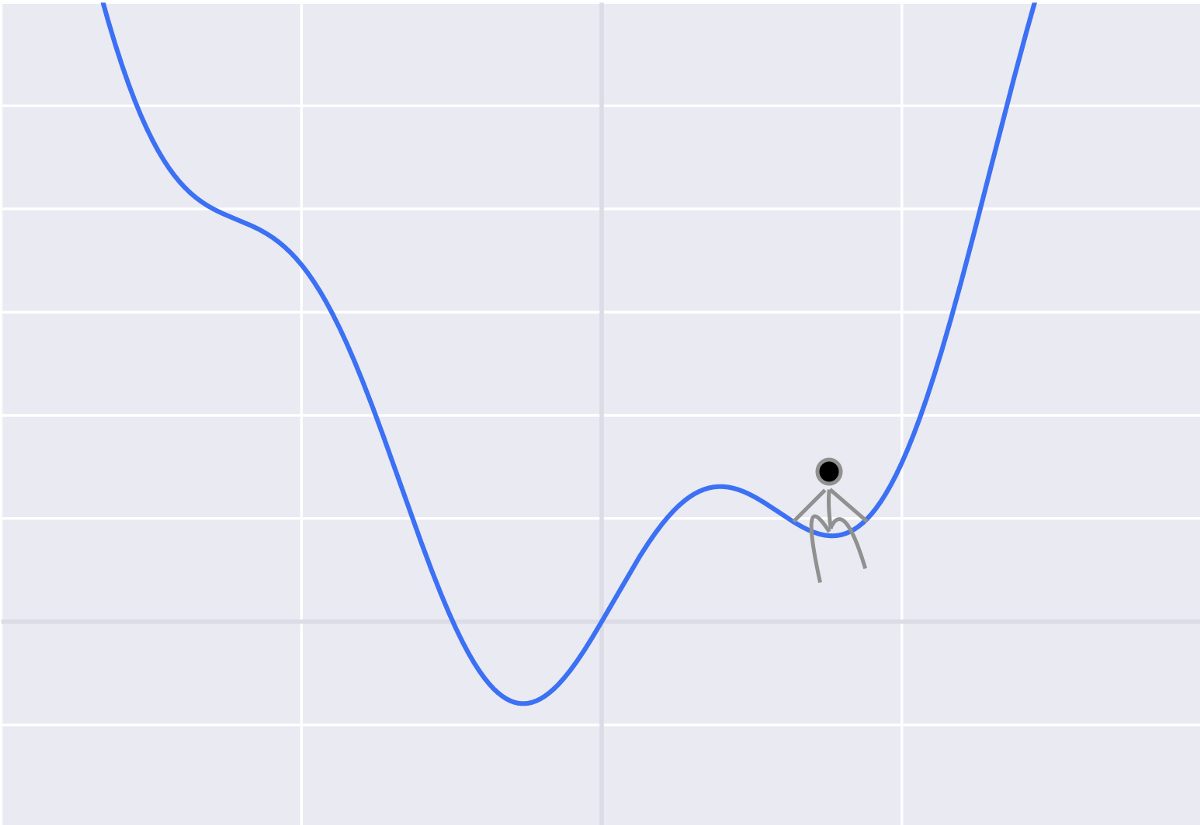
\includegraphics[width=0.6\paperwidth]{bob_local_chill.png}
\end{center}
\vfill %
\footnotesize 
\color{blue} \url{https://hackernoon.com/life-is-gradient-descent-880c60ac1be8}
\end{frame}


\begin{frame}{Седловые точки}
\begin{center}
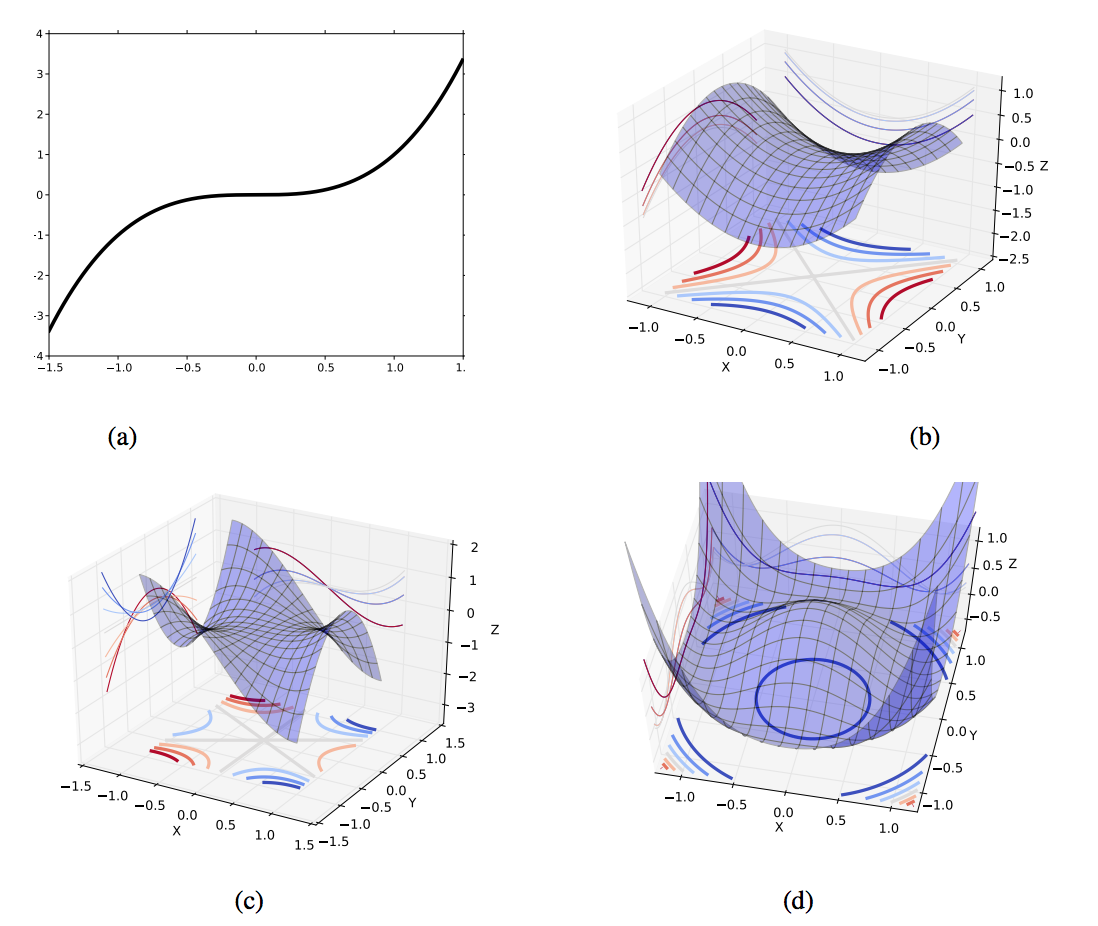
\includegraphics[width=0.5\paperwidth]{sedlo.png}
\end{center}
\vfill %
\footnotesize 
\color{blue} \url{https://arxiv.org/pdf/1406.2572.pdf}
\end{frame}


\begin{frame}{Визуализация потерь}
\begin{center}
	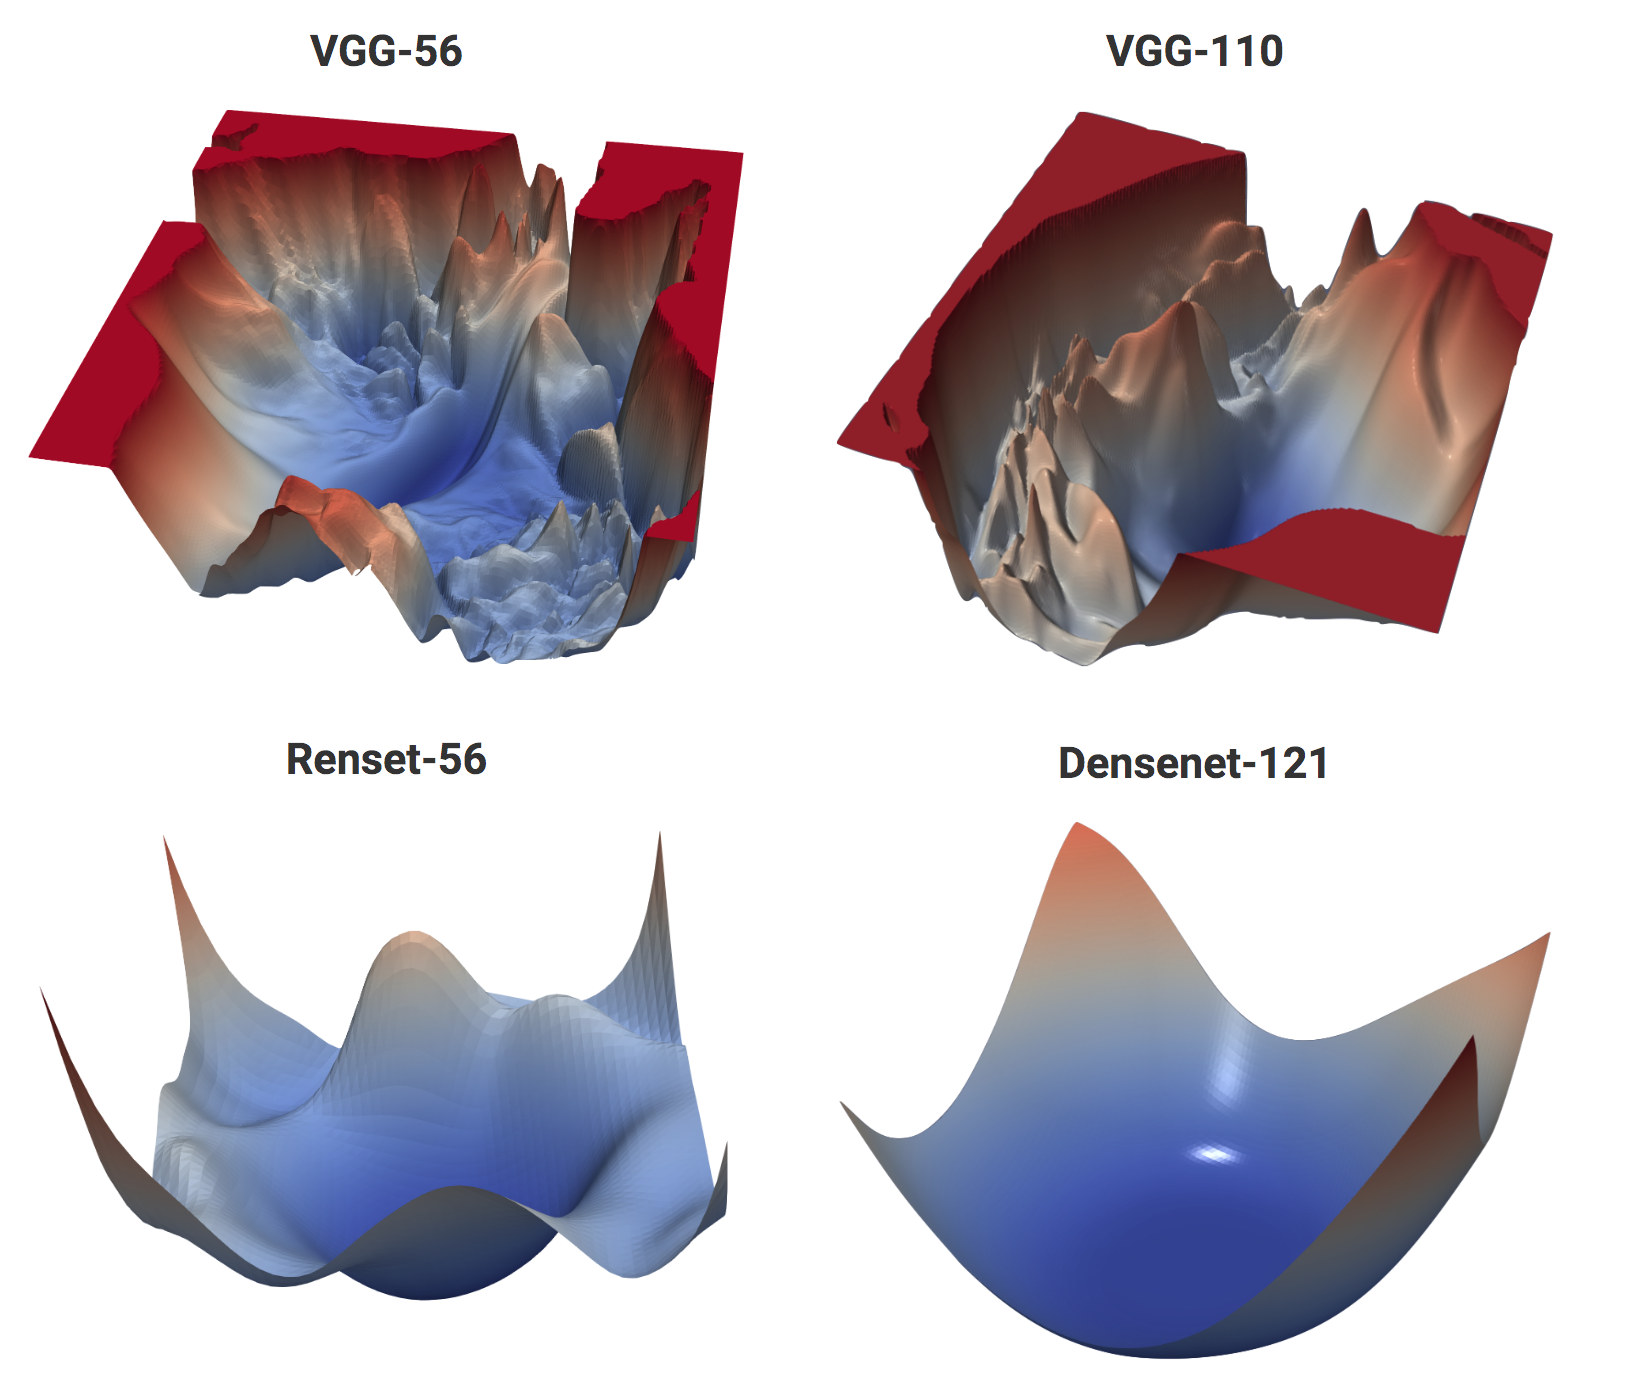
\includegraphics[width=0.5\paperwidth]{loss.png}
\end{center}
\vfill %
\footnotesize 
\color{blue} \url{https://arxiv.org/pdf/1712.09913.pdf} \newline  \url{https://github.com/tomgoldstein/loss-landscape}
\end{frame}



\begin{frame}{Циклическая скорость обучения (CLR)}
\begin{wideitemize}
	\item Хочется, чтобы был шанс вылезти из локального минимума, а также шанс сползти с седла $\Rightarrow$ давайте менять глобальную скорость обучения циклически
\end{wideitemize}
\begin{center}
	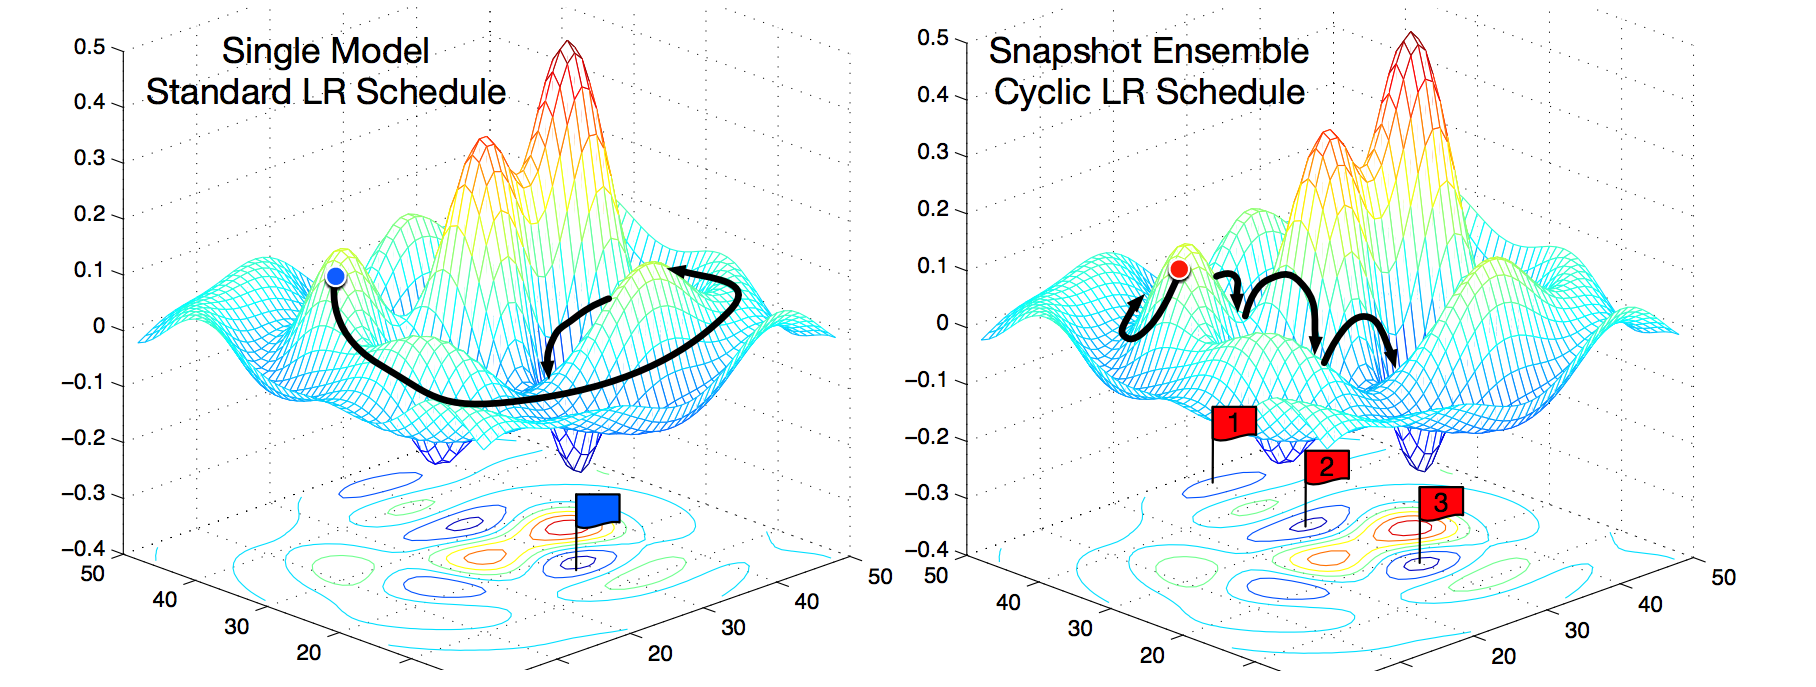
\includegraphics[width=0.7\paperwidth]{cycle_sgd.png}
\end{center}
\end{frame}


\begin{frame}{Циклическая скорость обучения (CLR)}
\begin{columns}[T] % align columns
	\begin{column}{.48\textwidth}
		\centering 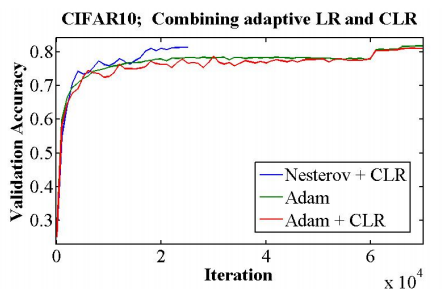
\includegraphics[scale=0.55]{cycle_2.png}
	\end{column}%
	\hfill%
	\begin{column}{.48\textwidth}
		\centering 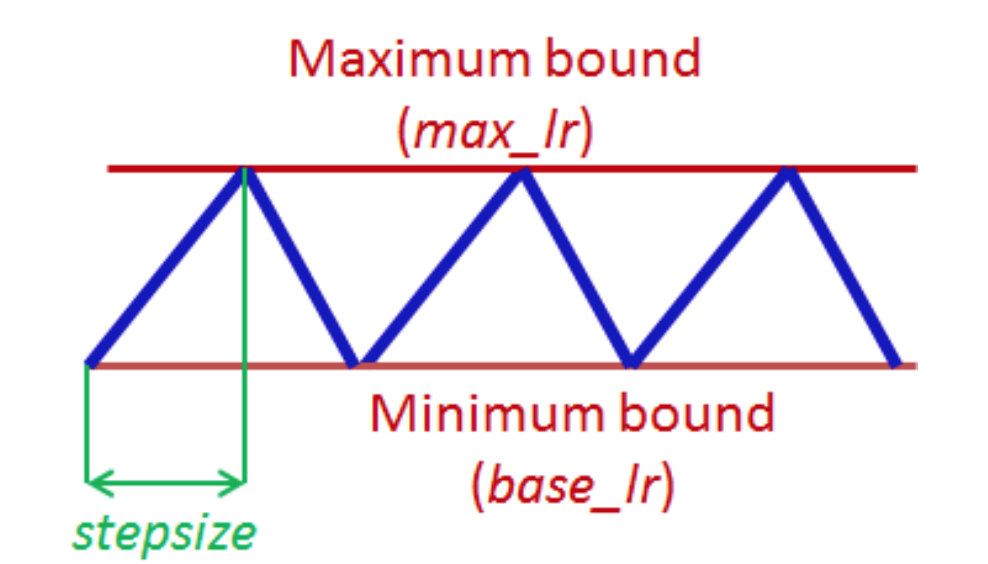
\includegraphics[scale=0.17]{cycle.png} \\ \mbox{ } \\
		Нестеров с CLR отработал \\ быстрее и лучше Adam \\ \alert{Нет одного правильного \\ алгоритма на все случаи!}  \\ Всегда надо экспериментировать
	\end{column}%
\end{columns}

\vfill %
\footnotesize  
\color{blue} \url{https://arxiv.org/pdf/1506.01186.pdf} \newline  \url{https://openreview.net/pdf?id=BJYwwY9ll}
\end{frame}



\begin{frame}{А что люди сейчас делают с оптимизаторами?}
\begin{wideitemize}
	\item  Нейросеть пытается сама от слоя к слою выстраивать новые, более сложные фичи
	\item Самостоятельно фичи больше придумывать не надо 
	\item При этом оптимизаторы какие-то слишком олдскульные и ручные 
	\item \alert{Круто было бы, если бы оптимизаторы тоже сами обучались}
	\item Такие работы в последнее время активно появляются, но какого-то суперпрогресса пока нет 
\end{wideitemize}

\vfill %
\footnotesize  
\color{blue} \url{https://arxiv.org/pdf/2009.11243.pdf}
\end{frame}



\begin{transitionframe}
	\begin{center}
		{\Huge Так как же обучить нейросетку?} \\ \mbox{ } \\
			\begin{tikzpicture}
			\node[inner sep=0pt] (russell) at (0,0)
			{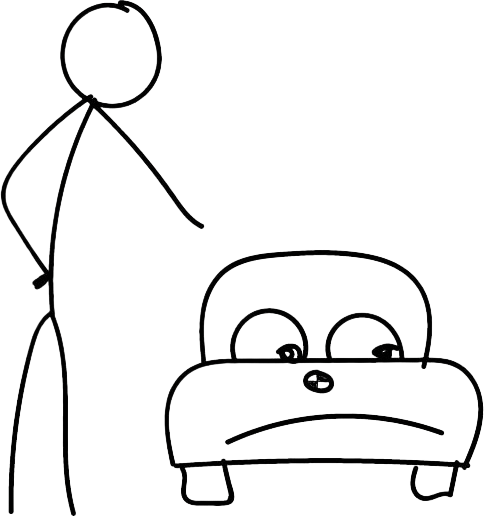
\includegraphics[scale = 0.15]{ml.png}};
			\node[] at (0,-0.6) {Ты необучаем!};
			\end{tikzpicture}
	\end{center}
\end{transitionframe}


\begin{frame}{Нейросеть —  сложная функция}
\begin{wideitemize}
\item Прямое распространение ошибки (forward propagation): 

\[ X \Rightarrow X \cdot W_1 \Rightarrow f(X \cdot W_1) \Rightarrow f(X \cdot W_1) \cdot W_2 \Rightarrow \ldots \Rightarrow \hat{y} \]

\item Считаем потери:

\[Loss = \frac{1}{2} (y - \hat y)^2\]

\item Для обучения нужно использовать градиентный спуск
\end{wideitemize}
\end{frame}


\begin{frame}{Как обучить нейросеть?}

\[ L(W_1, W_2) =  \frac{1}{2} \cdot (y - f(X \cdot W_1) \cdot W_2)^2\]

Секрет успеха в умении брать производную и градиентном спуске.

\[f(g(x))' = f'(g(x)) \cdot g'(x) \]

\begin{equation*} 
\begin{aligned} 
\frac{\partial L}{\partial W_2} &=   { \only<2>{ \color{red}} - (y - f(X \cdot W_1) \cdot W_2) } \cdot f(X \cdot W_1) \\
\frac{\partial L}{\partial W_1} &= { \only<2>{ \color{red}}  - (y - f(X \cdot W_1) \cdot W_2) } \cdot W_2 f'(X \cdot W_1) \cdot W_1 
\end{aligned}
\end{equation*}

\vfill

\only<2>{\alert{Дважды ищем одно и то же $\Rightarrow$ оптимизация поиска производных даст нам алгоритм обратного распространения ошибки (back-propagation)}}
\end{frame}


\begin{frame}{Back-propagation}
\begin{center}
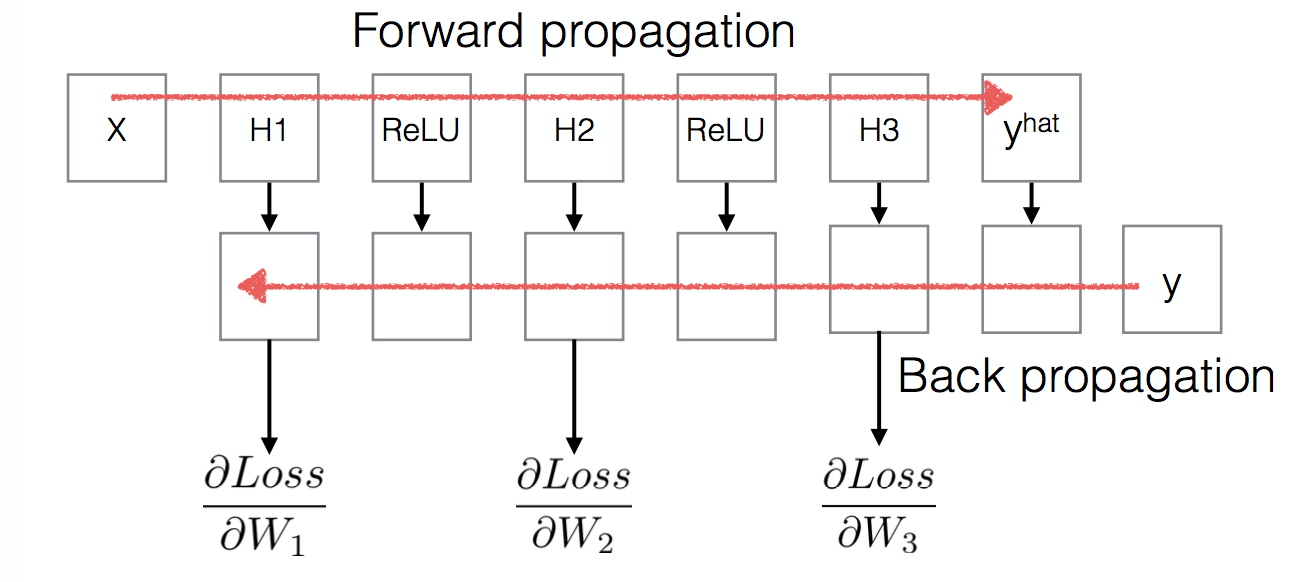
\includegraphics[width=.8\linewidth]{backpropagation.png}
\end{center}
\end{frame}


\end{document}

